\documentclass[11pt, oneside]{article}   	% use "amsart" instead of "article" for AMSLaTeX format
\usepackage{geometry}                		% See geometry.pdf to learn the layout options. There are lots.
\geometry{letterpaper}                   		% ... or a4paper or a5paper or ... 
%\geometry{landscape}                		% Activate for for rotated page geometry
%\usepackage[parfill]{parskip}    		% Activate to begin paragraphs with an empty line rather than an indent
\usepackage{graphicx}				% Use pdf, png, jpg, or eps� with pdflatex; use eps in DVI mode
								% TeX will automatically convert eps --> pdf in pdflatex		
\usepackage{amssymb}
\usepackage{amsmath}
\usepackage{parskip}
\usepackage{color}

\title{Plane and Sphere}
%\author{The Author}
%\section{}
% \subsection*{R code}
\date{}							% Activate to display a given date or no date

\graphicspath{{/Users/telliott_admin/Dropbox/Tex/png/}}

% \begin{center} 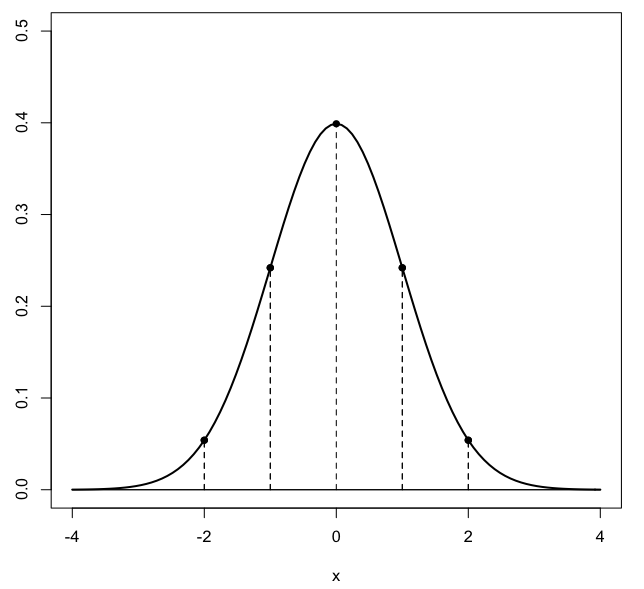
\includegraphics [scale=0.4] {gauss3.png} \end{center}
% \begin{bmatrix} a  &  b \\ c  &  d \end{bmatrix}
% \bigg |_

\begin{document}
\maketitle
\large
%\noindent

In Auroux's lecture (xx) he gives this problem:  we have the unit sphere centered at the origin, and a plane $x + y + z = 1$ which intersects the sphere.  The plane intersects all three axes at the same points where the sphere does, but it cuts off a little piece from the "northeast" top side, and we'd like to know some things about this piece.  It looks something like this
\vspace{5mm}
\begin{center} 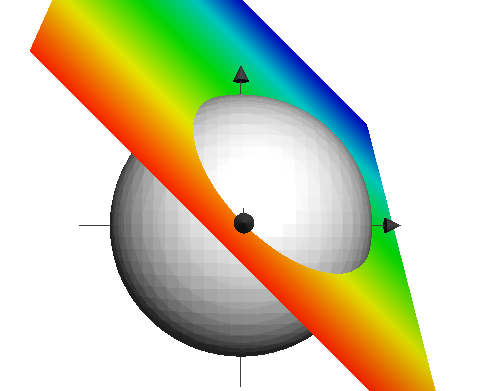
\includegraphics [scale=0.4] {spl.png} \end{center}

The intersection of a plane with a sphere is always a circle.  (Find the normal vector to the plane and extend a line of length $h$ from the origin to the plane along the normal.  From the point of intersection, extend any line along the plane to the intersection with the sphere.  The length of all such lines is the same, since one can draw a right triangle with sides consisting of the line, the radius of the sphere, and $h$). 

We know the normal vector to this plane from the coefficients of $xyz$, it is just $\langle 1,1,1 \rangle$.  We can find the point $P$ on the plane that is closest to the origin $O$ (it lies on a line parallel to the normal vector).  The parametric equation of this line is $P - O = t \ \mathbf{n}$.  Points on the line are of the form $(t,t,t)$.  So we want $ t + t + t = 1$, telling us that $t = 1/3$.

The point $(1/3,1/3,1/3)$ is on the normal vector starting from the origin, and it is on the plane.  The distance from $P$ to $O$ is $\sqrt{3 (1/3)^2}$, which equals $\frac{1}{\sqrt{3}}$.  The \emph{unit} normal vector is $\hat{\mathbf{n}} = \langle \frac{1}{\sqrt{3}},\frac{1}{\sqrt{3}},\frac{1}{\sqrt{3}} \rangle$.

Now, how about the volume?

One way to do this is to imagine the whole setup rotated so that $\hat{\mathbf{n}} \ || \ \hat{\mathbf{k}} $, and then integrate to find the volume.  If we set up the integral in cylindrical coordinates

\[ V = \iiint dV = \int_0^{2 \pi} \int_0^R \int \ dz \ r \ dr \ d \theta \]

We ask:  what are the bounds on $z$?  Clearly it starts at the plane ($z = \frac{1}{\sqrt{3}}$), and ends at $z=1-r$.  So then we have

\[ V = \iiint dV = \int_0^{2 \pi} \int_0^R \int_\frac{1}{\sqrt{3}}^{1-r} \ dz \ r \ dr \ d \theta \]
\[ = \int_0^{2 \pi} \int_0^R (1- \frac{1}{\sqrt{3}} - r) \ r \ dr \ d \theta \]
\[ = \int_0^{2 \pi} \int_0^R (\frac{1}{2})(1- \frac{1}{\sqrt{3}}) r^2 - \frac{1}{3} r^3 \ d \theta \]
\[ = 2 \pi\ [ \  (\frac{1}{2})(1- \frac{1}{\sqrt{3}}) R^2 - \frac{1}{3} R^3 \ ] \]

Another way to explore this problem is to find the intersection of the plane and the sphere by setting the two equations equal to each other using the variable $z$
\[ z = 1 - x - y = \sqrt{1 - x^2 - y^2} \]
Squaring both sides we get
\[ 1 - x - y -x + x^2 + xy - y + xy + y^2 = 1 - x^2 - y^2 \]
\[ 2x^2 + 2xy + 2y2 - 2x - 2y = 0 \]
\[ x^2 + xy + y^2 - x - y = 0 \]

We know this is a ellipse because (from the equation above we have that $A=1, B=1, C=1$  Since the discriminant, $B^2 - 4AC = -3$, and this is negative, we know that the equation is an ellipse.

Here is a plot:
\begin{center} 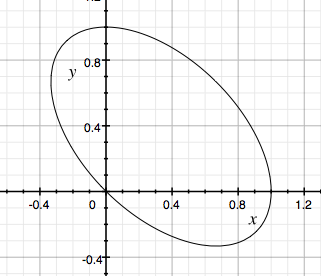
\includegraphics [scale=0.4] {spl2.png} \end{center}

What we're looking at is the projection of our circle onto the $xy$-plane.  Its center is at the projection of the point $P$ into the $xy$-plane  $(\frac{1}{3},\frac{1}{3})$.

If we could rotate this ellipse (by $\pi/4$) and translate it to the origin, we could get the radius of the circle (the projection is only squished along the line to the origin).  Or we can just go back to one of our first deductions and invoke Pythagoras
\[ r^2 + h^2 = R^2 = 1 \]
\[ h = \frac{1}{3} \]
\[ r = \sqrt{1-\frac{1}{9}} = \frac{2 \sqrt{2}}{3} \approx 0.94 \]

To actually do the rotation

\[ x = u\cos \theta + v\sin \theta \]
\[ y = -u\sin \theta + v\cos \theta \]
Since $\theta = \pi/4$
\[ \sin \theta = \cos \theta = \frac{1}{\sqrt{2}} \]

\[ x = \frac{u}{2} + \frac{v}{2} \]
\[ y = -\frac{u}{2} + \frac{v}{2} \]
Substituting
\[ x^2 = (\frac{u}{2} + \frac{v}{2})^2 = \frac{u^2}{4} + \frac{uv}{2} + \frac{v^2}{4} \]
\[ y^2 = (-\frac{u}{2} + \frac{v}{2})^2 = \frac{u^2}{4} - \frac{uv}{2} + \frac{v^2}{4} \]
\[ xy = (\frac{u}{2} + \frac{v}{2})(-\frac{u}{2} + \frac{v}{2}) = -\frac{u^2}{4} + \frac{v^2}{4} \]
Our equation is
\[ x^2 + xy + y^2 - x - y = 0 \]
Adding up the first three terms I get
\[ = \frac{u^2}{4} + 3\frac{v^2}{4} \]
with $x$ and $y$
\[ = \frac{u^2}{4} + 3\frac{v^2}{4} - \frac{u}{2} - \frac{v}{2} + \frac{u}{2} - \frac{v}{2} \]
\[ = \frac{u^2}{4} + 3\frac{v^2}{4} - v \]

???

\end{document}  